\chapter{Experiments}
\label{ch:experiments}

This chapter describes the experiments conducted for this work. First, the environments used for the experiments are described. Then the setup and goal is explained. And lastly, the results are shown and evaluated.

\section{Environments}
\label{sec:experiments:env}

Two of the environments used in this work come from the OpenAI gym robotics tasks. These are the FetchReach and the FetchPush environments. The third environment, called FetchPushBarrier, is a modification of the FetchPush environment. See figure \ref{fig:envs-overview} for an overview. All three environment share the same setup. The robot arm can be controlled with actions $a \in [-1,1]^4$. The first three dimensions of the vector control the movement of the arm along the axes. The fourth dimension allows to open and close the gripper. It is, however disabled for these environments to open the gripper. A value has to be provided nonetheless, but its value is ignored.

The goal in the FetchReach environment is to move the gripper to the red sphere. The FetchPush and FetchPushBarrier environments share the same goal of moving the black cube to the red sphere. The FetchPushBarrier environment has the added difficulty that the yellow barrier has to be avoided. The red sphere in all environments is only a marker for the target and has no physical body.

The FetchPush environment is slightly modified with an increased number of steps. The maximum is now 100 instead of the regular 50. This gives the agent room for small mistakes when moving the object.
\begin{figure}[btp]
    \centering
    \begin{subfigure}[b]{.32\textwidth}
        \centering
        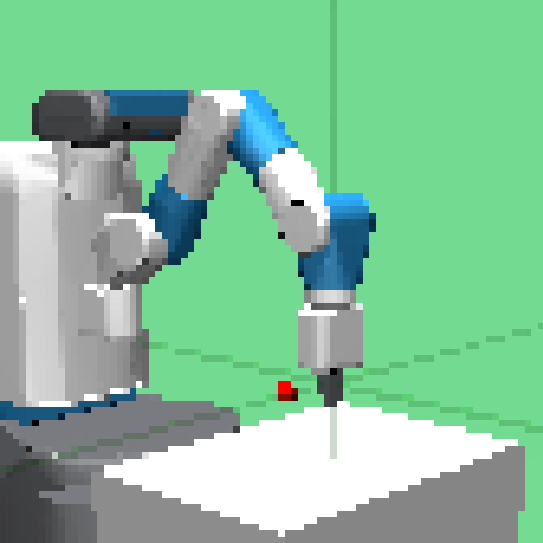
\includegraphics[width=\textwidth]{images/environments/fetch-reach-obs.png}
        \caption{FetchReach}
        \label{fig:envs:reach}
    \end{subfigure}
    \hfill
    \begin{subfigure}[b]{.32\textwidth}
        \centering
        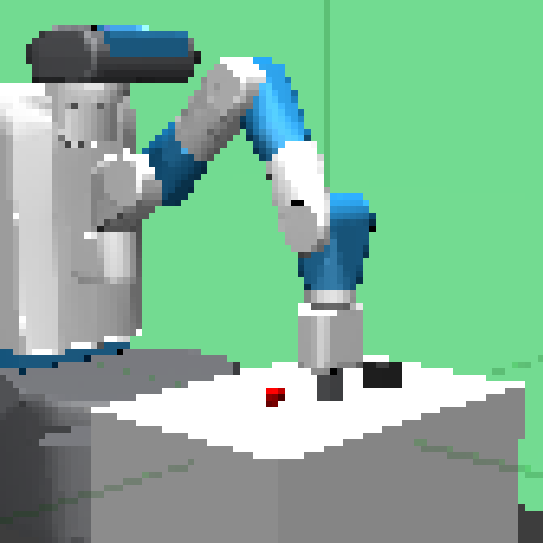
\includegraphics[width=\textwidth]{images/environments/fetch-push-obs.png}
        \caption{FetchPush}
        \label{fig:envs:push}
    \end{subfigure}
    \hfill
    \begin{subfigure}[b]{.32\textwidth}
        \centering
        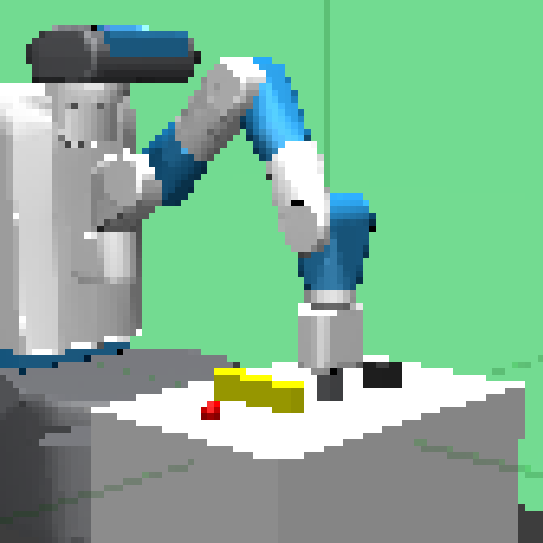
\includegraphics[width=\textwidth]{images/environments/fetch-push-barrier-obs.png}
        \caption{FetchPushBarrier}
        \label{fig:envs:barrier}
    \end{subfigure}
    \caption[Overview of the three environments used in this work.]{Overview of the three environments used in this work. The images show the actual $84\times84$ pixel observations the agents receive. The observations are a cropping of the original image, the gym Fetch environments render. See figure \ref{fig:env-axes} for the original image size.}
    \label{fig:envs-overview}
\end{figure}

\subsection{FetchPushBarrier}
\label{sec:environments:fetch-push-barrier}

The FetchPushBarrier environment is an adaptation of the regular FetchPush environment. The only things changed are the initialization to add a barrier and a cost function.

When initializing the FetchPushBarrier environment, first the gripper and the object are seeded the same as in the FetchPush environment. To position the barrier, first a random position along the x-axis is chosen. See figure \ref{fig:env-axes} for the naming of the axes. The position is drawn to let the barrier extend to the table edges at the most. To sample the placement along the y-axis, first it has to be determined if the barrier should be in front or behind the object, if seen from the camera. If the object is at the very front of the table, the barrier is always placed behind the object. If the object is at the very back, it is placed in front respectively. If the object is in the middle of the table, it is chosen at random if the barrier should be placed in front or behind the object. Afterwards, the exact placement along the y-axis is drawn at random, ensuring a minimum distance to the object, the gripper and the table edge. The size of the barrier is fixed and it is always position parallel to the axes.

After the barrier is placed, the position of the target is drawn at random. The placement is constrained in the y-axis to always be behind the barrier if seen from the object. In the x-axis, the position is constrained to the size of the barrier, to ensure that the object has to be moved around the barrier.

When taking a step in the environment, the reward is calculated just like in the FetchPush environment. For a dense reward, the negative distance between the object and the target is used. The sparse reward is $0$ if the distance between the goal and the target is below a threshold and $-1$ otherwise. Additionally a cost is computed after each step:
\begin{equation}
    C(s,a,s') = \begin{cases}
        0, &\quad\text{if } d \geq 0.1\\
        1-\frac{d}{0.1}, &\quad\text{else}\\
    \end{cases}
\end{equation}
Where $d$ is given by the minimum of the distances of the gripper and object to the barrier.

The maximum steps in the environment is increased to 150, to account for the added difficulty.

\begin{figure}[btp]
    \centering
        \begin{tikzpicture}
            \node at (0,0.3) (image)  {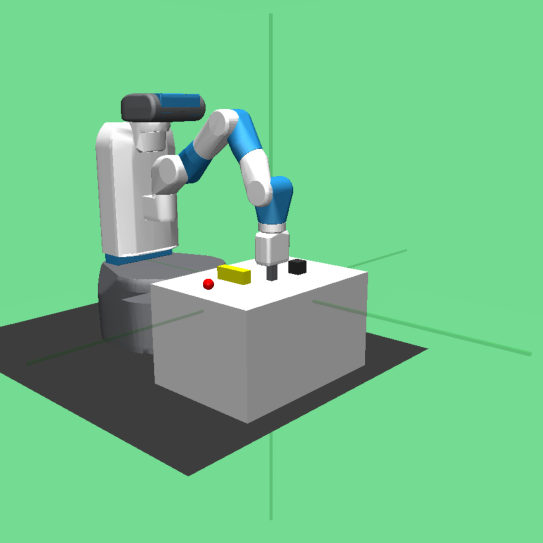
\includegraphics[width=.5\textwidth]{images/environments/fetch-push-barrier.png}};
            \draw[black, thick, ->] (0,0) -- (0,4.2) node[above] {$z$};
            \draw[black, thick, ->] (0,0) -- (4,-1) node[above] {$x$};
            \draw[black, thick, ->] (0,0) -- (4,1.3) node[above] {$y$};
        \end{tikzpicture}
    \caption{Axes in the FetchPushBarrier environment}
    \label{fig:env-axes}
\end{figure}

\section{Experiment Setup}
\label{sec:experiments:setup}

The goal with the experiments was to train an agent using frame stack observations for all three environments described in section \ref{sec:experiments:env}. The experiments use the training setup described in section \ref{sec:algo-high-dim-observations} with an ensemble teacher. This also includes the described option of augmenting the frame stacks with the gripper position to simplify the training. The high dimensional image observations consist of a stack of three frames. Each frame is an image of $84\times84$ colored pixels. 

First, for each environment, an ensemble of three SAC agents using the state was trained. If one of the agents was significantly worse than the others, more agents were trained and the best three picked for the ensemble. See table \ref{tab:ensemble-results} for the exact results of the ensemble agents. Afterwards, the agents using frame stacks or augmented observations are trained with the ensemble. All environments use a dense reward, i.e. a reward is not only given in the case of a success, but at each time step.

The machines used for training either used an Intel Core i9-9900K with 64 GiB of memory and a Nvidia RTX 2080 TI or an AMD Ryzen Threadripper 3960X with 130 GiB of memory and a Nvidia RTX A5000. CUDA version 11.6 was used with both GPUs.

\begin{table}[btp]
	\centering
	\begin{tabular}{lrrrrrr}
\toprule
Environment & Success Rate &     \makecell{Episode\\Reward} &     \makecell{Episode\\Cost} & \makecell{Mean\\Success Rate} & \makecell{Mean\\Reward} & \makecell{Mean\\Cost}\\
\midrule
\multirow{3}*{FetchReach}
 &        1.0 &  -0.600 &          & \multirow{3}*{1.0} & \multirow{3}*{-0.552}\\
 &        1.0 &  -0.572 &          \\
 &        1.0 &  -0.484 &          \\
\midrule
\multirow{3}*{FetchPush}
 &        0.930 &  -3.374 &          & \multirow{3}*{0.901} & \multirow{3}*{-4.134}\\
 &        0.849 &  -4.774 &          \\
 &        0.925 &  -4.253 &          \\
\midrule
\multirow{3}*{FetchPushBarrier}
 &        0.726 & -14.873 & 1.370 & \multirow{3}*{0.761} & \multirow{3}*{-14.083} & \multirow{3}*{1.58}\\
 &        0.790 & -12.439 & 1.075 \\
 &        0.767 & -14.937 & 2.294 \\
\bottomrule
\end{tabular}
	\caption[Overview of the results from all ensembles used in training.]{Overview of the results from all ensembles used in training. All agents were evaluated over 1000 episodes. The same seed was used for all environments.}
	\label{tab:ensemble-results}
\end{table}

\section{Results}
\label{sec:experiments:results}

The following section contains the results of the experiments made during this work. Experiments were made in the environments FetchReach, FetchPush and FetchPushBarrer. The most experiments were made in the FetchReach environment. Training setups that do not perform well in this environment are expected to not have meaningful results in the much harder FetchPush and FetchPushBarrier environments. Therefore some setups were omitted for these environments. The results shown in this section are, if not otherwise stated, averaged over 3 trainings with different random seeds.

\subsection{FetchReach}
\label{sec:results:fetch-reach}

The FetchReach environment is fairly easy and was therefore chosen as a starting point for the experiments in this work. As table \ref{tab:ensemble-results} shows, the three agents of the ensemble for the teacher are all able to solve the task each time. The agents using image observations were trained with regular SAC and SAC together with the two improvements described in section \ref{sec:preliminaries-high-dim-observations}, autoencoders and DrQ. All algorithms were trained with only frame stacks and frame stacks augmented with the gripper position. Additionally, all algorithms were trained with and without the teacher. The $\alpha$ value that defines the importance of the teacher is set to one. This results in a total of 12 combinations. The success rates during training of all 12 setups are plotted in figure \ref{fig:results:reach}. The success rate of SAC state is added as reference. The episode rewards during training are plotted in figure \ref{fig:results:reach-reward}. It does, however, not make sense to compare the rewards of the setups with and without a teacher, since the preference reward algorithm uses reward shaping. Additionally, all agents were evaluated on 1000 episodes. The mean success rate and reward can be seen in table \ref{tab:results:reach}.

The training setups using DrQ were all able to reliably solve the task and they are also the only ones to do so. Adding the gripper information to the observations did, however, increase the sample efficiency. The same is even more true for adding a teacher. Combined, this results in the DrQ agent using augmented states and a teacher almost being as efficient as SAC state. The mean rewards from the evaluation show a similar pattern. The reward is always higher when adding a robot or a teacher. Since the environment uses dense rewards, i.e. the distance between the gripper and the target at each time step, this indicates that the agents are able to solve the task faster.

For the setups using the SAC and SAC-AE algorithms, the picture is not quite as clear. Plain SAC does not benefit from adding the gripper information. Adding a teacher, however, significantly increases the success rate and sample efficiency. SAC-AE benefits from the gripper information and the teacher. Using the teacher results in a higher success rate than adding the gripper information. However, if the gripper information is added to the observations, also adding the teacher does not further increase the success rate. The success rate is actually lower that using SAC-AE with a teacher but without the gripper information. A possible explanation for this lies in the architecture of the SAC-AE agent. The autoencoder only uses the frame stack and tries to reproduce it. It does not benefit from the added gripper information. It also does not benefit from the reward shaping through the teacher, as the autoencoder uses a reconstruction loss and is independent from the reward. This is in contrast to the actor and critic that both benefit from the gripper information and the teacher. This difference could lead to very different updates on the shared CNN encoder during training and could explain the discrepancy in the success rate. The fact that the SAC-AE+robot+teacher setup is outperformed by the same setup without the autoencoder supports this theory.

When looking at the episode reward in figure \ref{fig:results:reach-reward}, it is clear, that DrQ has the highest reward in all setups. This is consistent with the success rate of the DrQ setups. Also, it can be seen that when using a teacher, also adding the gripper information to DrQ increases the sample efficiency.
The episode rewards for the setups using plain SAC and SAC-AE are very similar. Again, this is consistent with the success rates. The success rates of the SAC and SAC-AE setups with a teacher are fairly similar to each other. The same is true for the setups without a teacher.

In general, it can be said that adding a teacher always lead to improvements in the success rate or the sample efficiency over the base version of the algorithm. In fact, for all three algorithms, the best training setup uses a teacher.

\begin{figure}
    \centering
    \begin{subfigure}[b]{.32\textwidth}
        \centering
        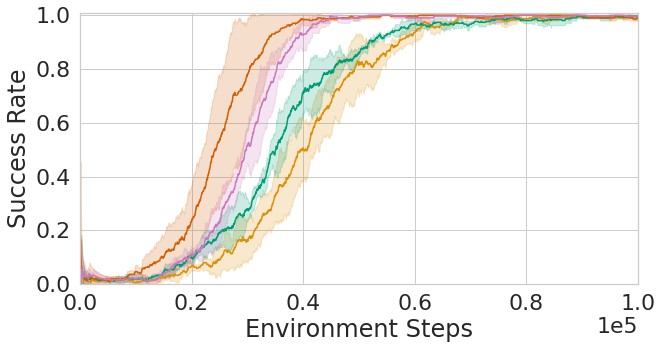
\includegraphics[width=\textwidth]{images/results/reach/drq.png}
        \caption{DrQ}
        \label{fig:results:reach:drq}
    \end{subfigure}
    \hfill
    \begin{subfigure}[b]{.32\textwidth}
        \centering
        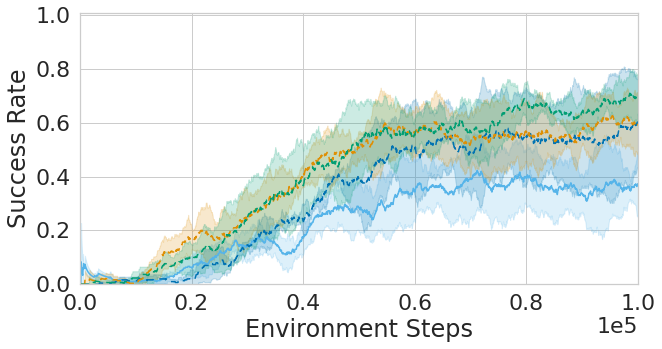
\includegraphics[width=\textwidth]{images/results/reach/sacae.png}
        \caption{SAC-AE}
        \label{fig:results:reach:sacae}
    \end{subfigure}
    \hfill
    \begin{subfigure}[b]{.32\textwidth}
        \centering
        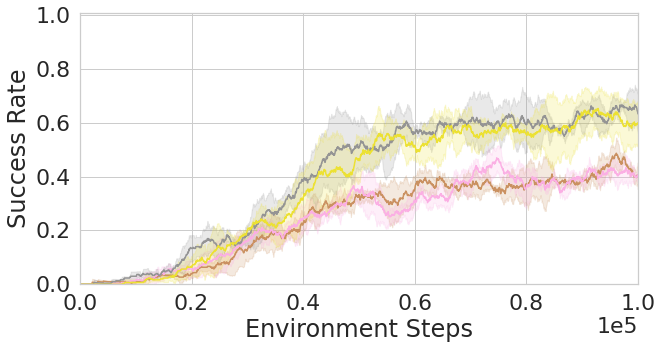
\includegraphics[width=\textwidth]{images/results/reach/sac.png}
        \caption{SAC Pixel}
        \label{fig:results:reach:sac}
    \end{subfigure}
    \hfill
    \begin{subfigure}[b]{.99\textwidth}
        \centering
    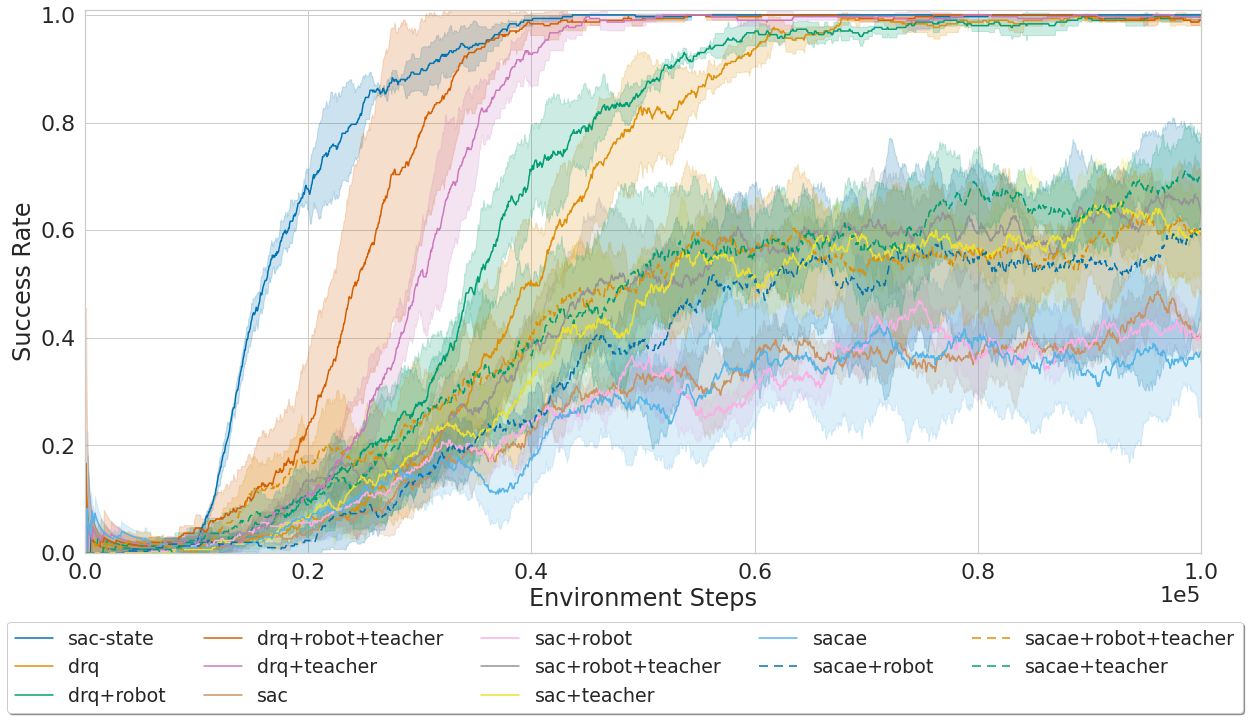
\includegraphics[width=\textwidth]{images/results/reach/all.png}
        \caption{All FetchReach experiments}
        \label{fig:results:reach:all}
    \end{subfigure}
    \caption[The success rates from all experiments on the FetchReach environment.]{The success rates from all experiments on the FetchReach environment. The algorithms SAC pixel, SAC autoencoder and DrQ were each trained with and without augmented states and teachers. As a reference, SAC state is added. The subplots (\subref{fig:results:reach:drq})-(\subref{fig:results:reach:sac}) each show the success rates for one algorithm.}
    \label{fig:results:reach}
\end{figure}

\begin{figure}
    \centering
    \begin{subfigure}[b]{\textwidth}
        \centering
        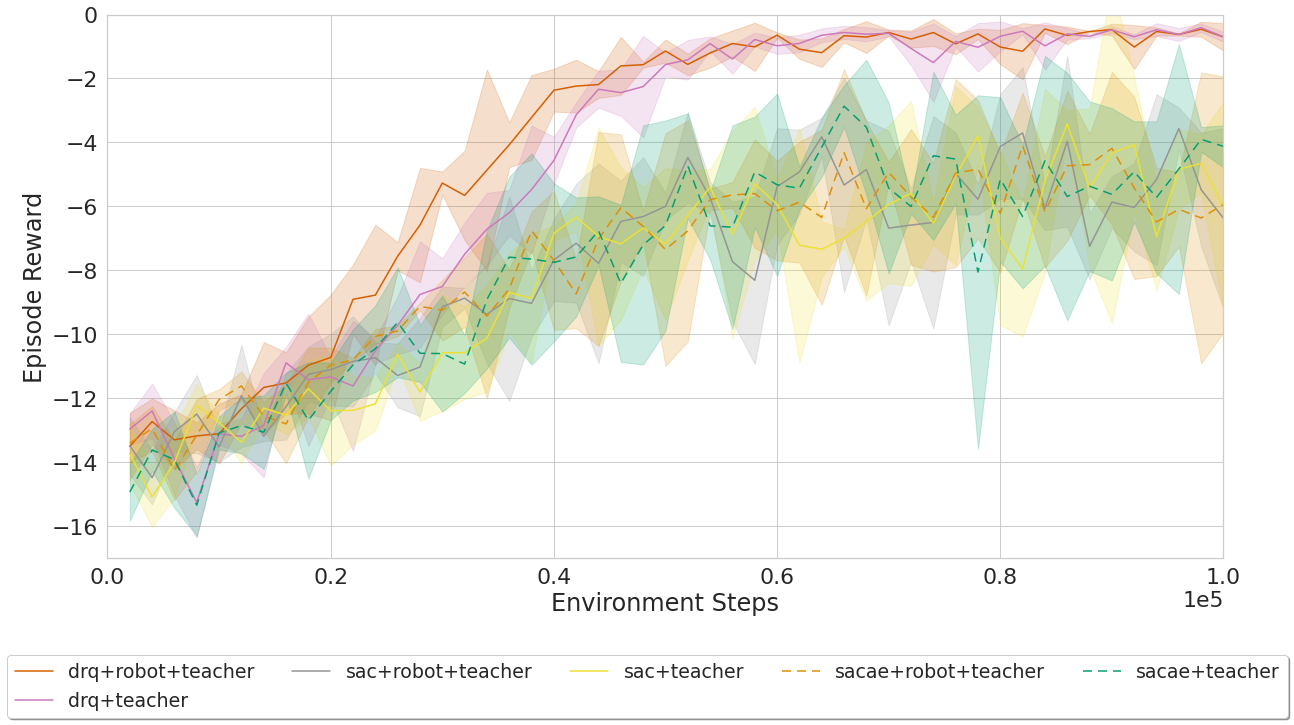
\includegraphics[width=\textwidth]{images/results/reach/reward_teacher.png}
        \caption{Episode reward with a teacher}
        \label{fig:results:reach:reward-teacher}
    \end{subfigure}
    \hfill
    \begin{subfigure}[b]{\textwidth}
        \centering
        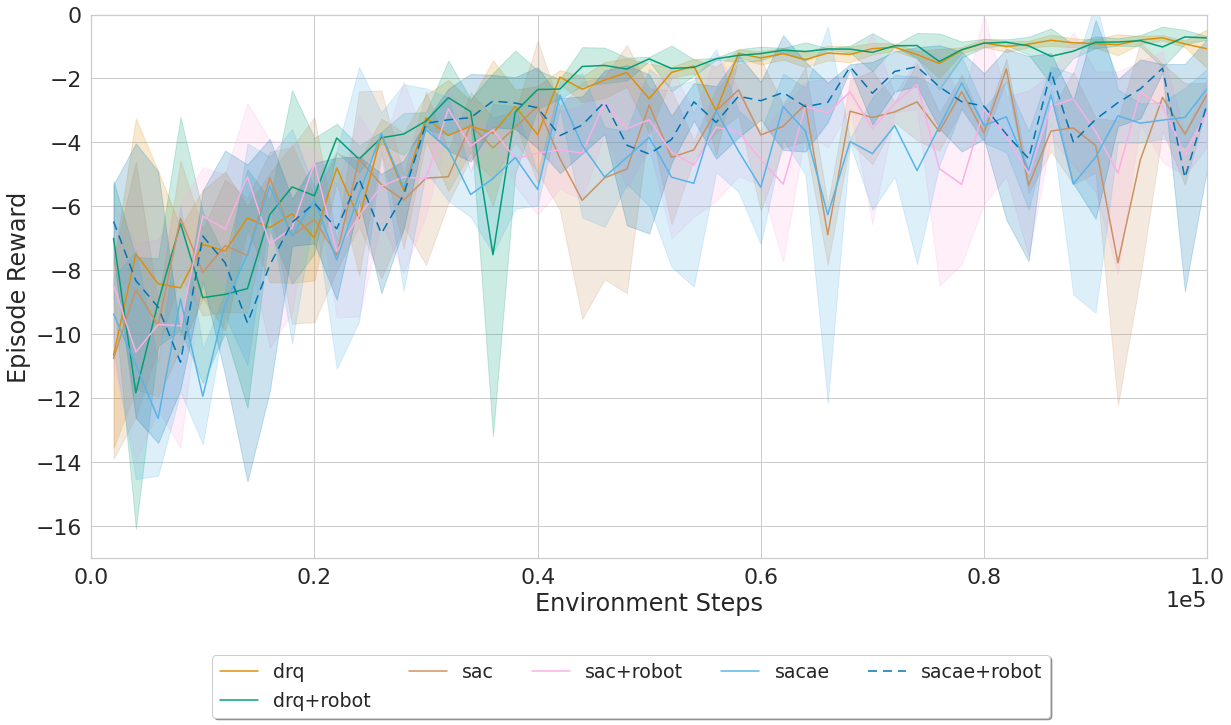
\includegraphics[width=\textwidth]{images/results/reach/reward_no_teacher.png}
        \caption{Episode reward without a teacher}
        \label{fig:results:reach:reward_no_teacher}
    \end{subfigure}
    \caption[The episode rewards from all experiments on the FetchReach environment.]{The episode rewards from all experiments on the FetchReach environment. The algorithms SAC pixel, SAC autoencoder and DrQ were each trained with and without augmented states and teachers. Since the preference reward algorithm uses reward shaping, it does not make sense to compare the experiments with and without a teacher.}
    \label{fig:results:reach-reward}
\end{figure}

\begin{table}[btp]
    \centering
    \begin{tabular}{lllrr}
\toprule
Algorithm & Robot & Teacher & Mean Success Rate & Mean Episode Reward \\
\midrule
\multirow{4}{*}{drq} & \multirow{2}{*}{False} & False &             0.994 &      -0.852 \\
      &      & True &             0.994 &      -0.720 \\
\cline{2-5}
      & \multirow{2}{*}{True} & False &             0.993 &      -0.763 \\
      &      & True &             0.996 &      -0.698 \\
\cline{1-5}
\cline{2-5}
\multirow{4}{*}{sac} & \multirow{2}{*}{False} & False &             0.425 &      -3.360 \\
      &      & True &             0.608 &      -2.945 \\
\cline{2-5}
      & \multirow{2}{*}{True} & False &             0.393 &      -3.622 \\
      &      & True &             0.628 &      -2.912 \\
\cline{1-5}
\cline{2-5}
\multirow{4}{*}{sacae} & \multirow{2}{*}{False} & False &             0.388 &      -3.484 \\
      &      & True &             0.657 &      -2.787 \\
\cline{2-5}
      & \multirow{2}{*}{True} & False &             0.573 &      -2.882 \\
      &      & True &             0.588 &      -3.084 \\
\bottomrule
\end{tabular}
    \caption[Mean success rate and reward for all agents trained on the FetchReach environment.]{Mean success rate and reward for all agents trained on the FetchReach environment. The shown values are the mean over the three agents trained for each setup. All agents were evaluated on 1000 episodes. The environments were initialized with the same seed. The preference reward algorithm is not used during evaluation. Therefore, the reward shown here is the environment reward.}
    \label{tab:results:reach}
\end{table}

\subsection{FetchPush}
\label{sec:results:fetch-push}

Only agents trained with DrQ were able to reliably solve the FetchReach environment. Since the FetchPush environment is significantly harder than the FetchReach environment, all agents were trained with DrQ. Additionally, the robot state augmentations were used for all experiments. Again, this is based on the experience with FetchReach, where this improved the sample efficiency.

Experiments were conducted with and without a teacher. When a teacher was used, the fixed $\alpha$ values of $1.0$ and $0.5$ were tried. Additionally, an adaptive $\alpha$ was used as described in section \ref{sec:adaptive-alpha}. The adaptive $\alpha$ is based on the environment reward. To stabilize the adaptive $\alpha$ value, it is calculated from a moving average of the environment reward for one episode with a coefficient of $0.01$. The $\alpha$ value was then given by the following function:
\[
\alpha(r_{env}) = \begin{cases}
        1, &\quad\text{if } r_{env} < -20\\
        1-\frac{-20-r_{env}}{-20}, &\quad\text{else}\\
    \end{cases}
\]
With this function, the $\alpha$ value starts at one at the beginning of the training and gets lower once the agent surpasses an environment reward of $-20$ per episode. At a non achievable environment reward of zero, the $\alpha$ value would also reach zero.

Figure \ref{fig:results:push-success} shows the success rates during training of all experiments. The different $\alpha$ values of the experiments with a teacher and their development during training are plotted in figure \ref{fig:results:push-alpha}. The rewards during training are not shown here, as all experiments use different $\alpha$ values and the rewards are therefore not comparable. All trained agents were evaluated on 1000 episodes. The mean success rates and episode rewards can be seen in table \ref{tab:results:push}.

When looking at the success rate of the experiment without a teacher, it is clearly visible that there is no noticeable training effect. The success rate does not change over the course of the training. The way the FetchPush environment is initialized, it is possible for the object and the target to touch each other from the beginning. The environment is therefore sometimes solved without the robot moving the object. Most likely this is why the success rate is not zero when training without the teacher.

When training with a fixed $\alpha$ of one, the agents were able to solve the task in roughly $40\%$ of the cases during training. When evaluated over 1000 episodes, the mean success rate was $40.3\%$. The success rate of the agents trained with an $\alpha$ of $0.5$ increased a little slower that the one with an $\alpha$ of one, but surpassed it at some point. During training, a success rate of up to $70\%$ was reached. However, the success rate shows some fluctuation. In the final evaluation, the success rate was $61.5\%$. During training, the success rate is calculated based on the last 100 episodes. The final evaluation is calculated using 1000 episodes. This explains the difference in the results. A possible explanation for the higher success rate with a lower $\alpha$ lies in the quality of the teacher. As it can be seen in table \ref{tab:ensemble-results}, the ensemble, the teacher consists of, has a mean success rate of $90.1\%$. With an $\alpha$ of one, the agent in training can only learn to imitate the teacher. If, however, the teacher is not acting perfectly, the agent will learn subpar actions. With a lower $\alpha$ value, the agent gets direct feedback from the environment an can also learn from this.

With the adaptive $\alpha$ we saw a success rate very similar to the experiments with a fixed $\alpha$ of 0.5. Figure \ref{fig:results:push-alpha} shows the development of the $\alpha$ value over the course of the training. The adaptive value dropped significantly below the fixed value of 0.5. However, this did not lead to changes in the success rate. In the final evaluation, we see a slight improvement of the agents with an adaptive $\alpha$ over the ones with a fixed $\alpha$ of 0.5, with regards to both the success rate and the mean episode reward.

One problem that might lower the performance with the adaptive $\alpha$ lies in the architecture of Off-policy RL algorithms in combination with the preference reward algorithm. While both the environment reward $r_{env}$ and the teacher reward $r_{teacher}$ are in range $[0,1]$, it is possible that $r_{teacher}$ is significantly higher than $r_{env}$. This can happen especially if $r_{env}$ is very small for each step. When $r_{env}$ increases and the $\alpha$ is reduced, this can lead to overall lower values of the preference reward $r_{pr}$, although the agent is performing better. Since the replay buffer only stores $r_{pr}$, the agent then learns the wrong behavior. A possible solution for this would be to store both $r_{env}$ and $r_{teacher}$ and only calculate $r_{pr}$ when it is needed for the training, using the current $\alpha$ value. However, this possible improvement was left for future works, due to time restricitions.

Overall, the adaptive $\alpha$ slightly improved the performance. However, the main benefit is that it gives us a different way to set the importance of the teacher. It can be hard to set a good $\alpha$ value. With the adaptive $\alpha$, we instead have to set a reward threshold when to start lowering the $\alpha$ value. Note that this is only one possibility to adapt the $\alpha$ value. Other functions may be used as well.

\begin{figure}
    \centering
    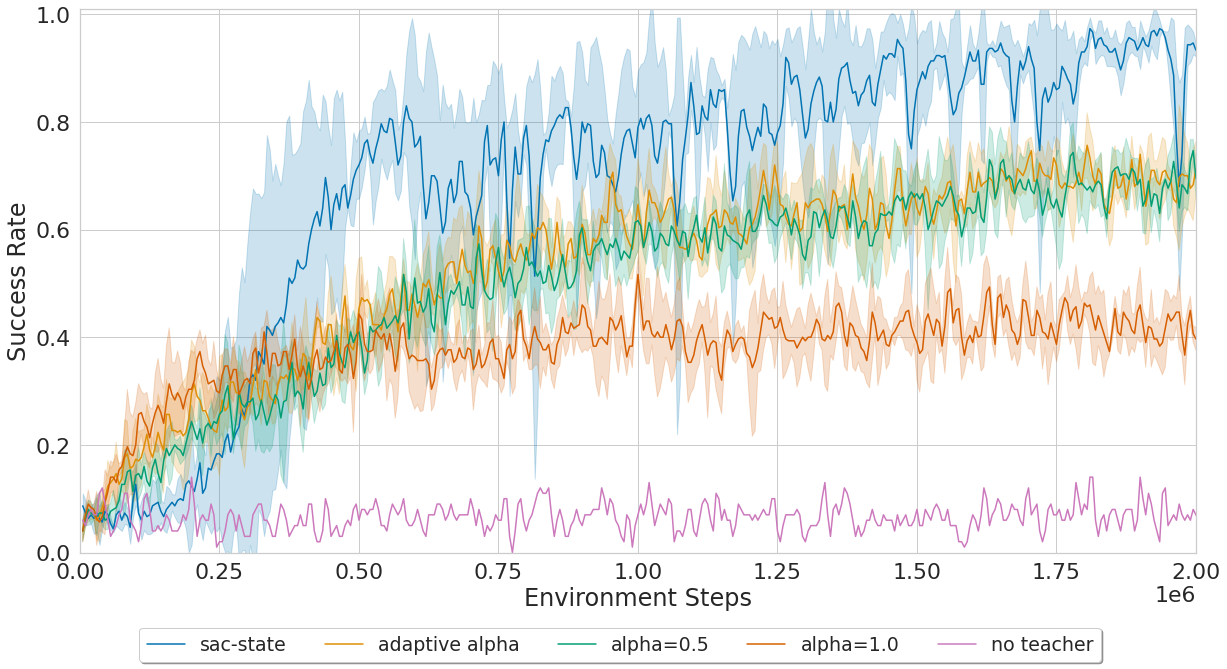
\includegraphics[width=\textwidth]{images/results/push/success_rate.png}
    \caption[The success rates from all experiments on the FetchPush environment.]{The success rates from all experiments on the FetchPush environment. All agents were trained with DrQ and the robot state augmentations. As a reference, SAC state is added. In contrast to the other experiments, the agent without a teacher was only trained with one seed. It is however clearly visible that there is no noticeable training effect.}
    \label{fig:results:push-success}
\end{figure}
\begin{figure}
    \centering
    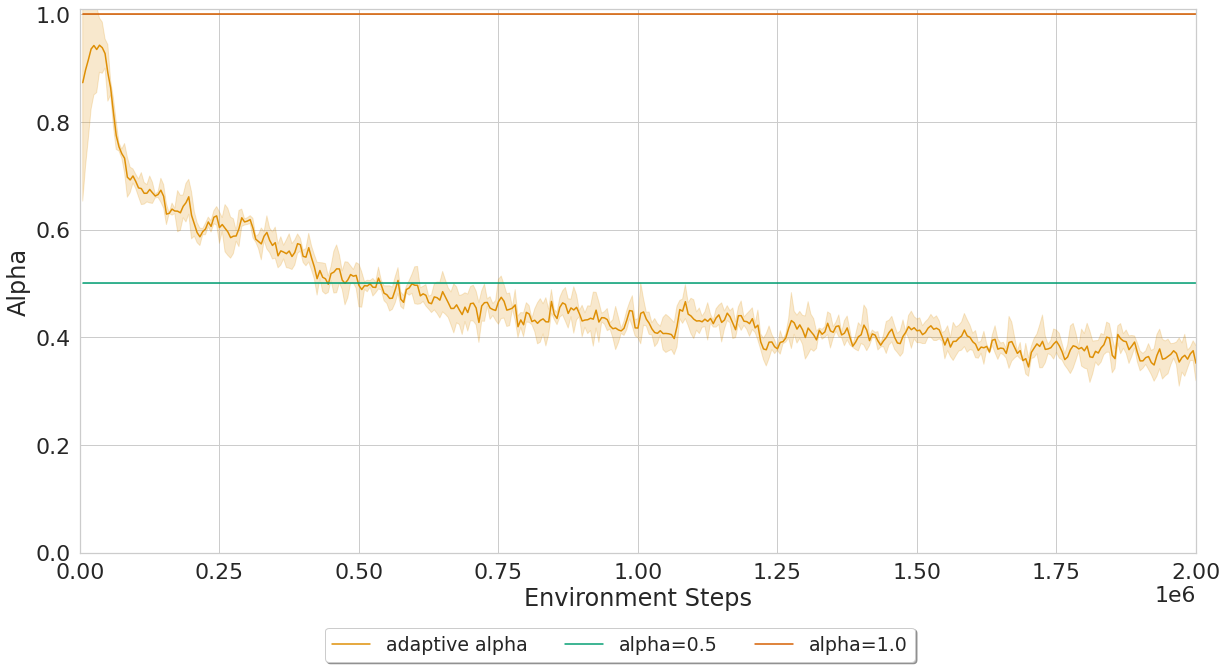
\includegraphics[width=\textwidth]{images/results/push/alpha.png}
    \caption[The $\alpha$ value from all experiments on the FetchPush environment.]{The $\alpha$ value from all experiments on the FetchPush environment. The $\alpha$ value of the experiments with an adaptive $\alpha$ is calculated with a function based on the environment reward. See section \ref{sec:adaptive-alpha} for reference.}
    \label{fig:results:push-alpha}
\end{figure}

\begin{table}[btp]
    \centering
    \begin{tabular}{lrr}
\toprule
Experiment & Mean Success Rate & Mean Episode Reward \\
\midrule
Adaptive $\alpha$ &             0.617 &              -7.641 \\
$\alpha$=0.5      &             0.615 &              -8.338 \\
$\alpha$=1.0      &             0.403 &             -11.269 \\
No teacher     &             0.071 &             -17.316 \\
\bottomrule
\end{tabular}


    \caption[Mean success rate and reward for all agents trained on the FetchPush environment.]{Mean success rate and reward for all agents trained on the FetchPush environment. The shown values are the mean over the three agents trained for each setup. All agents were evaluated on 1000 episodes. The environments were initialized with the same seed. The preference reward algorithm is not used during evaluation. Therefore, the reward shown here is the environment reward.}
    \label{tab:results:push}
\end{table}

\subsection{FetchPushBarrier State}
\label{sec:results:fetch-push-barrier-state}

As described in section \ref{sec:environments:fetch-push-barrier}, the FetchPushBarrier environment is an adaptation from the FetchPush environment that adds a cost function. To represent the cost, the three methods from section \ref{sec:safety}, reward based, safety training, and safety evaluation, were used. The parameters $\lambda_r$ and $\lambda_c$ that define the importance of the reward and the cost in the reward based approach were both set to one. All agents were trained using the state space as observations. 

Figure \ref{fig:results:barrier-state-success} shows the success rate and figure \ref{fig:results:barrier-state-cost} the cost during training. To show the effect of the safety evaluation, the agents were evaluated every 25000 training steps. The figures \ref{fig:results:barrier-state-cost-train} and \ref{fig:results:barrier-state-cost-eval} show the cost during training and periodic evaluation respectively. For the periodic evaluation, the safety evaluation was used with the parameter $n=10$ and $\delta=0.05$. The parameter $n$ defines how many actions are sampled from the policy for each action that is needed from the agent. The parameter $\delta$ defines the threshold when to select the action that is expected to maximize the reward or minimizes the cost. Additionally, all agents were evaluated on 1000 episodes. The results are shown in table \ref{tab:results:barrier-state}. The values are averaged over the three agents trained with each algorithm.

When looking at the success rate, all algorithms show a similar sample efficiency. However, the safety training shows a higher success rate than the reward based approach. The safety evaluation performed worse than the reward based approach. In the final evaluation, the safety training and the reward based approach have very similar success rates of $68\%$ and $67.5\%$.

The cost during training, as plotted in figure \ref{fig:results:barrier-state-cost-train} shows a similar picture. Again, the safety training performs the best, followed by the reward based approach. The high cost from the safety evaluation was expected, as only the reward is optimized during training with the safety evaluation. In the final evaluation, the safety training clearly outperforms the reward based approach with a mean cost of $1.757$ against $3.115$. With the safety training there is also a clearly visible training effect with regards to the cost. The cost gets lower, the further the training progressed. With the reward based approach, the training effect is not quite as visible. This might be due to the fact that the final cost is not as good. When looking at the cost during the periodic evaluation, the safety evaluation clearly lowered the costs, but is still significantly worse than the two other approaches. Also the cost seem to be very similar over the course of the training after a short period with lower costs. This could be explained with the way the FetchPushBarrier  environment works. To produce costs, the agent first needs to learn to move the object towards the target, since the barrier is always located between the object and the target. As the agent improves, it will more often come into states were costs are possible, mitigating the effect of the improved avoidance of costs.

\begin{figure}
    \centering
    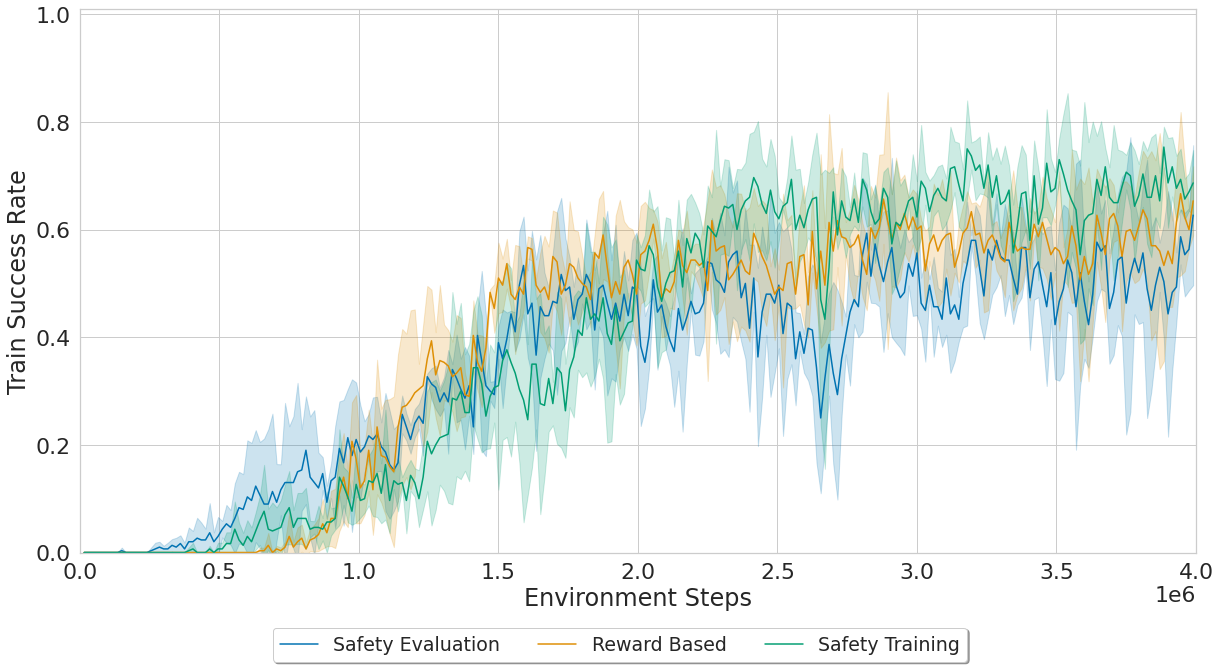
\includegraphics[width=\textwidth]{images/results/push-barrier-state/success.png}
    \caption[The success rates from on the FetchPushBarrier state experiments.]{The success rates from the FetchPushBarrier state experiments. The FetchPushBarrier environment was trained with the reward based approach as well as the safety training and safety evaluation algorithm.}
    \label{fig:results:barrier-state-success}
\end{figure}

\begin{figure}
    \centering
    \begin{subfigure}[b]{\textwidth}
        \centering
        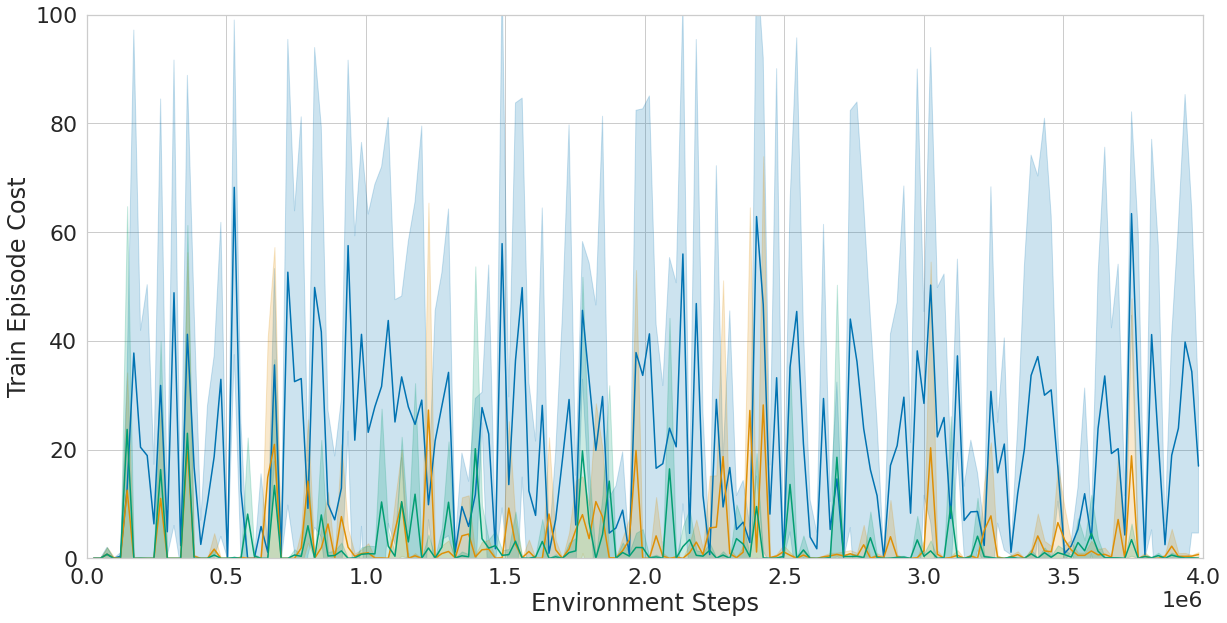
\includegraphics[width=\textwidth]{images/results/push-barrier-state/cost.png}
        \caption{Episode cost during training}
        \label{fig:results:barrier-state-cost-train}
    \end{subfigure}
    \hfill
    \begin{subfigure}[b]{\textwidth}
        \centering
        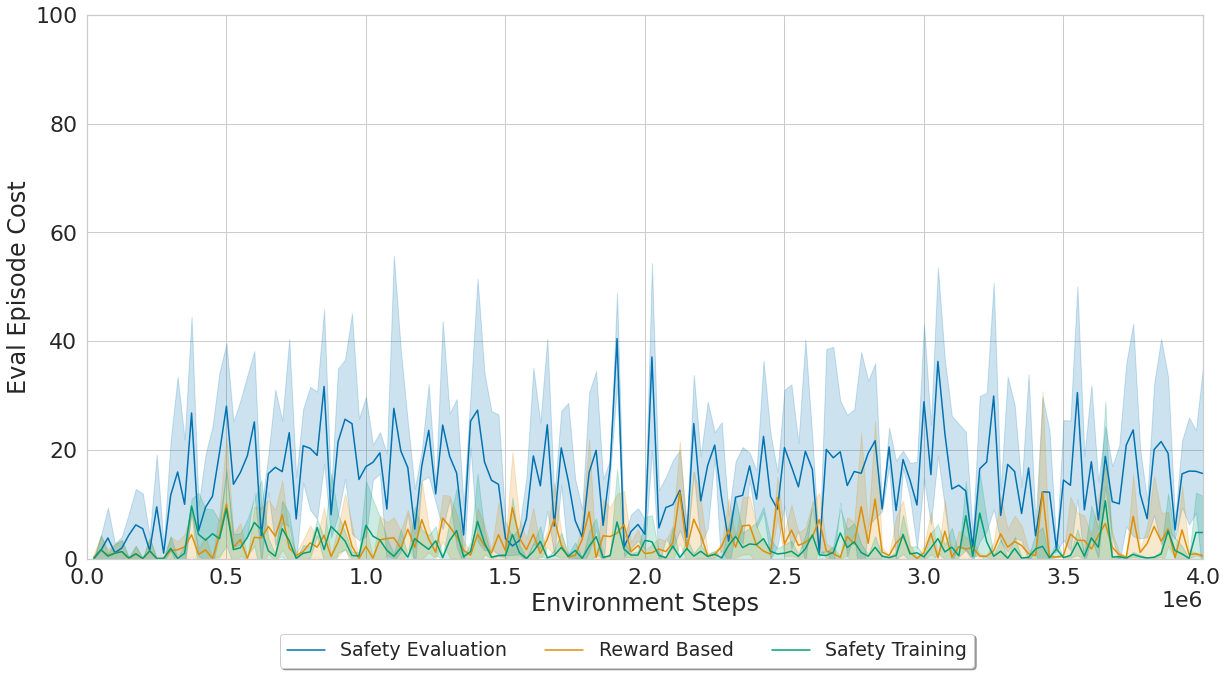
\includegraphics[width=\textwidth]{images/results/push-barrier-state/eval_cost.png}
        \caption{Episode cost from periodic evaluation during training}
        \label{fig:results:barrier-state-cost-eval}
    \end{subfigure}
    \caption[The episode cost from the FetchPushBarrier state experiments.]{The episode cost from the FetchPushBarrier state experiments. The FetchPushBarrier environment was trained with the reward based approach as well as the safety training and safety evaluation algorithm. During the training, the agents were periodically evaluated. Subplot (\subref{fig:results:barrier-state-cost-train}) shows the costs during training and subplot (\subref{fig:results:barrier-state-cost-eval}) the cost during the evaluation. The safety evaluation used the parameters $n=10$ and $\delta=0.05$.}
    \label{fig:results:barrier-state-cost}
\end{figure}

\begin{table}[btp]
    \centering
    \begin{tabular}{lrrr}
\toprule
Algorithm & Mean Success Rate & Mean Reward & Mean Cost \\
\midrule
Reward Based      &             0.675 &     -16.466 &     3.115 \\
Safety Evaluation deactivated      &             0.551 &     -15.710 &    21.057 \\
Safety Evaluation activated &             0.576 &     -15.498 &    16.069 \\
Safety Training   &             0.680 &     -13.278 &     1.757 \\
\bottomrule
\end{tabular}
    \caption[Mean success rate, reward and cost for all agents trained on the FetchPushBarrier environment using state.]{Mean success rate and reward for all agents trained on the FetchPushBarrier environment using state. The shown values are the mean over the three agents trained for each setup. All agents were evaluated on 1000 episodes. The safety evaluation agents were evaluated with the parameters $n=10$ and $\delta=0.05$. This choice of parameters resulted in the lowest mean episode cost with the safety evaluation.}
    \label{tab:results:barrier-state}
\end{table}

The three agents trained for the safety evaluation were additionally evaluated with different values for $n$ and $\delta$. For $n$, the values 1, 2, 5, and 10 were used. For $\delta$ the values 0.05, 0.1, 0.2, and 0.5. Not that for $n=1$ the choice of $\delta$ does not matter. Each agent was evaluated for 1000 episodes with each parameter combination. Table \ref{tab:results:barrier-state-safety-eval} shows the mean success rate, episode reward and episode cost for each parameter combination. The mean is calculated over the results from the three agents. Additionally, the results are visualized in figure \ref{fig:results:barrier-state-safety-eval}.

It is clearly visible that a higher value for $n$ results in a lower cost. This is easily explained with the way the algorithm works. The algorithm samples $n$ actions from the actor. With a higher value for $n$, the probability to get a low cost action is higher. However, a higher value also results in a longer execution time. Therefore, the parameter $n$ has to be chosen with a trade-off between cost and execution time. Drawing more sample also slightly increased the success rate. This can be explained by the stochastic nature of the actors. The more actions are drawn the higher the probability to get a good action. However, since the action with the lowest expected cost is selected, the effect on the success rate is only marginal. When looking at the mean episode reward, the difference between the experiments is so little that an interpretation makes no sense.

The value for $\delta$ seems to make no difference in all of the experiments. This is explained by a misconception when designing this evaluation. The choices for $\delta$ are within the range of the cost of one action, while the safety critic learns the expected cost for a whole episode. Therefore, the expected cost is always higher than $\delta$ and the action with the lowest expected cost is selected.

Overall, it can be said that the safety evaluation was able to reduce the cost, with a trade-off between the cost and the execution time. However, the cost is still a lot higher than the cost produced by an agent trained with the safety training algorithm or the reward based approach.

\begin{figure}
    \centering
    \begin{subfigure}[b]{.49\textwidth}
    \centering
    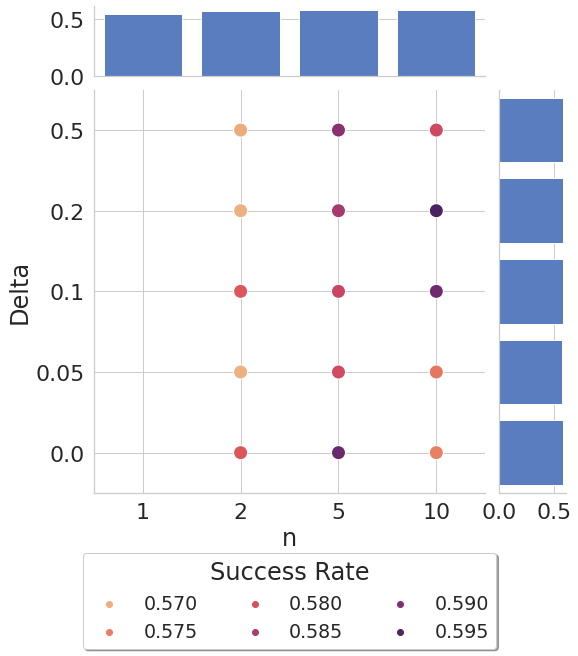
\includegraphics[width=\textwidth]{images/results/push-barrier-state/safety_eval_success.png}
    \caption{Safety evaluation success rate}
    \label{fig:results:barrier-state-safety-eval-success}
    \end{subfigure}
    \hfill
    \begin{subfigure}[b]{.49\textwidth}
    \centering
    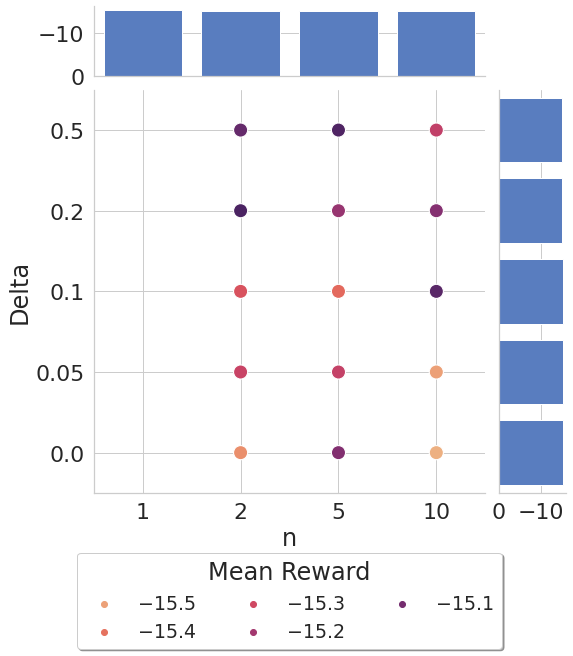
\includegraphics[width=\textwidth]{images/results/push-barrier-state/safety_eval_reward.png}
    \caption{Safety evaluation reward}
    \label{fig:results:barrier-state-safety-eval-reward}
    \end{subfigure}
    \hfill
    \begin{subfigure}[b]{.6\textwidth}
    \centering
    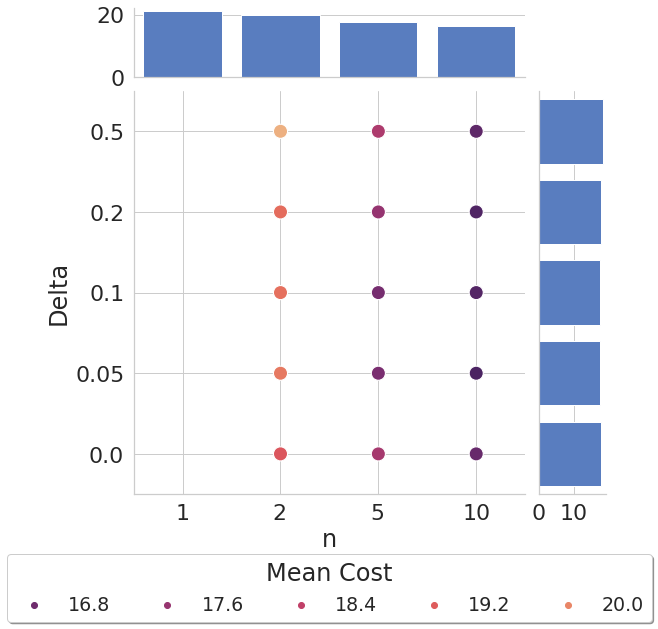
\includegraphics[width=\textwidth]{images/results/push-barrier-state/safety_eval_cost.png}
    \caption{Safety evaluation reward}
    \label{fig:results:barrier-state-safety-eval-cost}
    \end{subfigure}
    \caption[Analysis of the safety evaluation algorithm.]{Analysis of the safety evaluation algorithm with different values for $n$ and $\delta$. The three agents trained for safety evaluation were each evaluated with the different parameters. For $n=1$ the value of $\delta$ makes no difference. The subplots (\subref{fig:results:barrier-state-safety-eval-success})-(\subref{fig:results:barrier-state-safety-eval-cost}) show the success rate, mean reward and mean cost for all parameter combinations. The bar plots on the side show the mean values for the specific values for $n$ or $\delta$, averaged over the other parameter.}
    \label{fig:results:barrier-state-safety-eval}
\end{figure}

\begin{table}[btp]
    \centering
    \begin{tabular}{llrrr}
\toprule
n & $\delta$ & \makecell{Mean\\Success Rate} & \makecell{Mean\\Episode Reward} & \makecell{Mean\\Episode Cost} \\
\midrule
1  &   -  &             0.550 &     -15.608 &    21.177 \\
\cline{1-5}
\multirow{5}{*}{2} & 0.00 &             0.579 &     -15.460 &    19.089 \\
   & 0.05 &             0.570 &     -15.280 &    19.756 \\
   & 0.10 &             0.579 &     -15.329 &    19.588 \\
   & 0.20 &             0.570 &     -15.004 &    19.510 \\
   & 0.50 &             0.570 &     -15.065 &    20.797 \\
\cline{1-5}
\multirow{5}{*}{5} & 0.00 &             0.592 &     -15.125 &    17.886 \\
   & 0.05 &             0.581 &     -15.273 &    17.024 \\
   & 0.10 &             0.582 &     -15.382 &    16.939 \\
   & 0.20 &             0.586 &     -15.174 &    17.564 \\
   & 0.50 &             0.589 &     -15.014 &    18.023 \\
\cline{1-5}
\multirow{5}{*}{10} & 0.00 &             0.575 &     -15.531 &    16.647 \\
   & 0.05 &             0.576 &     -15.498 &    16.069 \\
   & 0.10 &             0.592 &     -15.038 &    16.259 \\
   & 0.20 &             0.596 &     -15.132 &    16.198 \\
   & 0.50 &             0.581 &     -15.264 &    16.464 \\
\bottomrule
\end{tabular}


    \caption[Analysis of the safety evaluation algorithm.]{Analysis of the safety evaluation algorithm with different values for $n$ and $\delta$. The three agents trained for safety evaluation were each evaluated with the different parameters. For $n=1$ the value of $\delta$ makes no difference. The values shown here are the mean of the three agents.}
    \label{tab:results:barrier-state-safety-eval}
\end{table}

\subsection{FetchPushBarrier Pixel}
\label{sec:results:fetch-push-barrier-pixel}

\begin{table}[btp]
    \centering
    \begin{tabular}{llrrr}
\toprule
Algorithm & $\alpha$   & \makecell{Mean\\Success Rate} & \makecell{Mean\\Episode Reward} & \makecell{Mean\\Episode Cost} \\
\midrule
\multirow{2}{*}{Reward Based} & 0.5 &             0.003 &     -45.532 &     2.425 \\
                & 1.0 &             0.003 &     -52.985 &     6.809 \\
\cline{1-5}
\multirow{2}{*}{Safety Training} & 0.5 &             0.003 &     -40.041 &     3.080 \\
                & 1.0 &             0.001 &     -46.977 &     2.220 \\
\bottomrule
\end{tabular}
    \caption[Mean success rate, reward and cost for all agents trained on the FetchPushBarrier environment using pixels.]{Mean success rate and reward for all agents trained on the FetchPushBarrier environment using pixels. For each setup only one agent was trained. All agents were evaluated on 1000 episodes.}
    \label{tab:results:barrier-drq}
\end{table}

The final experiment was conducted on the FetchPushBarrier environment using image observations. It uses the combination of the preference reward algorithm and a cost representation. Experiments were conducted with the reward based approach and the safety training, as these had the highest success rates in the previous experiments. When using the reward based approach, first the reward and cost are combined and then the preference reward is calculated. Unlike in definition \ref{def:preference-reward}\ref{enm:pr:external-reward}, the environment reward $r_{env}$ is not given by the MDPs reward function, but by the combination of the reward and the cost function $R_{cost}(s,a,s')$. See equation \ref{eq:reward-based-cost} for the definition of the function. The combined reward function is then given by:
\[
r_{pr} = \alpha * r_{teacher} + (1-\alpha) * \big(\lambda_r R(s,a,s') - \lambda_c C(s,a,s')\big)
\]
Again, the parameters $\lambda_r$ and $\lambda_c$ for the reward based approach were both set to one. We trained agents using $\alpha$ values of $0.5$ and one. The parameter $\alpha$ defines the importance of the teacher in contrast to the environment reward.

After the training, we evaluated the agents on 1000 episodes. The results are shown in table \ref{tab:results:barrier-drq}. None of the agents was able to reach a meaningful success rate. However, all of the agents where able to solve the task at least once. In contrast to the FetchPush environment, the FetchPushBarrier environment is always initialized in a way that requires the agent to move the object to solve the task. This indicates that the agents did learn some behavior required to solve the task but not quite how to solve it. This theory is supported when looking at videos from the evaluation. Figure \ref{fig:results:barrier-drq-frames} shows 5 frames from a video recorded during the evaluation of the agent trained with safety training and an $\alpha$ of $0.5$. The agent learned to move the object around the barrier and towards the target, but does not move it quite far enough. The episode is therefore not considered a success.

For the sake of completeness, figure \ref{fig:results:barrier-drq-cost} shows the development of the cost during the training. However, since the goal for the agents is to solve the task while keeping the cost low, it makes little sense to interpret the cost if the task is not solved. An agent that does not move the object and always keeps a distance to the barrier could achieve minimal cost, but would never solve the task. Because there is little to interpret with regards to the result for this experiment, we only trained one agent for each parameter combination.

We see two reasons why we were not able to reliably solve the FetchPushBarrier environment using high dimensional image observations. The first reasons is the difficulty of the environment itself. Even when training on state observations, our agents where only able to reach a mean success rate of $68\%$. The second reason is connected to the first. The teacher we used is an ensemble of SAC state agents. We trained six agents in total using SAC state and selected the three best agents. By doing so, we were able to increase the mean success rate of the teacher to $76.1\%$. This can be seen in table \ref{tab:ensemble-results}. However, this is significantly worse than the teacher for FetchReach and FetchPush. Figure \ref{fig:results:barrier-drq-ensemble-bar} shows the success rates in relation to each other. Additionally, it shows the mean confidence of the teachers. To calculate the mean confidence, first the best agent of each ensemble, with regards to the success rate, was selected. This agent was evaluated on 1000 episodes. For each action, the confidence was calculated using all three agents. The mean of the confidence of all actions is shown in the chart. The teacher for the FetchPushBarrier environment also has the lowest mean confidence. This means that the agents of the ensemble propose different actions as the best action. However, this makes it hard for the student to learn the best action. The most drastic example would be, if two of the teacher agents want to pass the barrier on different sides. It is up to future work to show if an improved teacher can lead to better performance on the FetchPushBarrier environment using high dimensional image observations.

\begin{figure}
    \centering
    \begin{subfigure}[b]{.19\textwidth}
    \centering
    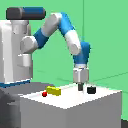
\includegraphics[width=\textwidth]{images/results/push-barrier-drq/frames/frame_0.png}
    \end{subfigure}
    \begin{subfigure}[b]{.19\textwidth}
    \centering
    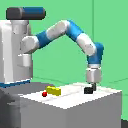
\includegraphics[width=\textwidth]{images/results/push-barrier-drq/frames/frame_1.png}
    \end{subfigure}
    \begin{subfigure}[b]{.19\textwidth}
    \centering
    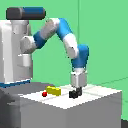
\includegraphics[width=\textwidth]{images/results/push-barrier-drq/frames/frame_2.png}
    \end{subfigure}
    \begin{subfigure}[b]{.19\textwidth}
    \centering
    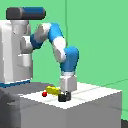
\includegraphics[width=\textwidth]{images/results/push-barrier-drq/frames/frame_3.png}
    \end{subfigure}
    \begin{subfigure}[b]{.19\textwidth}
    \centering
    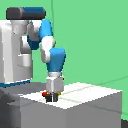
\includegraphics[width=\textwidth]{images/results/push-barrier-drq/frames/frame_4.png}
    \end{subfigure}
    \hfill
    \caption[Frames from a video recorded on the FetchPushBarrier - Pixel environment]{Frames from a video recorded on the FetchPushBarrier - Pixel environment. The video was recorded with the agent trained using safety training and an $\alpha$ of $0.5$. Between each image, 5 frames where skipped.}
    \label{fig:results:barrier-drq-frames}
\end{figure}

\begin{figure}[btp]
    \centering
    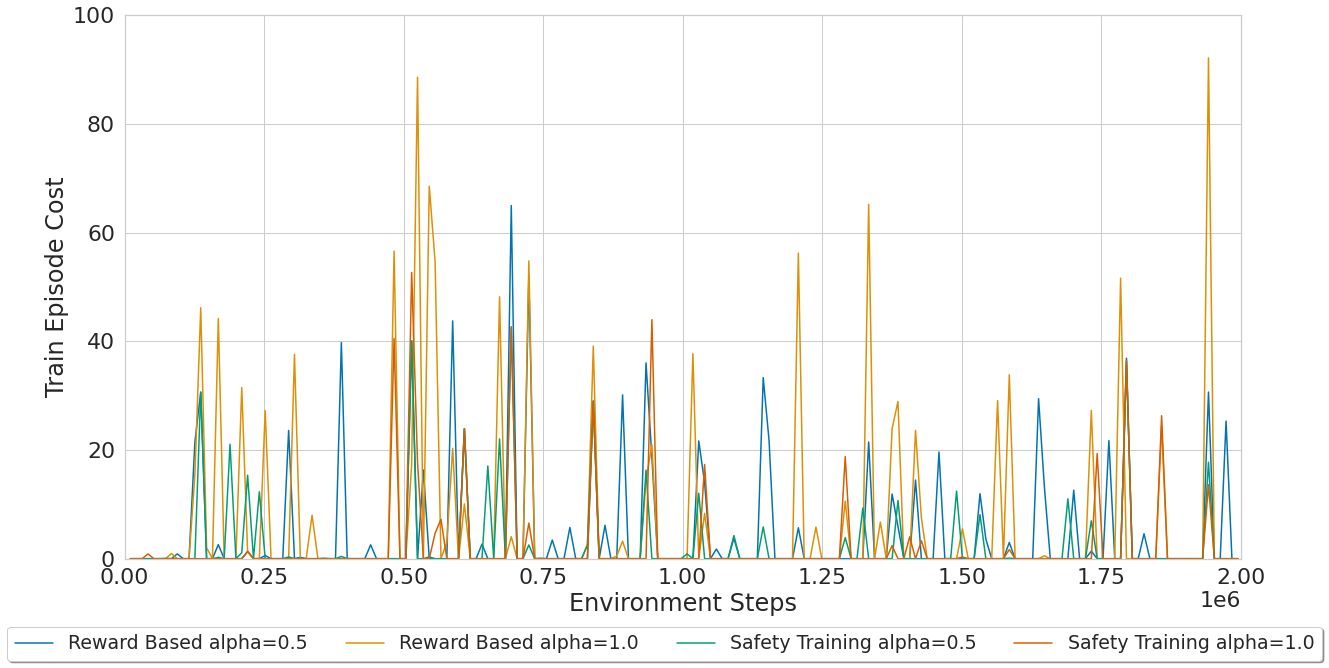
\includegraphics[width=\textwidth]{images/results/push-barrier-drq/cost.png}
    \caption[The episode cost from the FetchPushBarrier pixel experiments.]{The episode cost from the FetchPushBarrier pixel experiments. The FetchPushBarrier environment was trained with the reward based approach as well as the safety training.}
    \label{fig:results:barrier-drq-cost}
\end{figure}

\begin{figure}
    \centering
    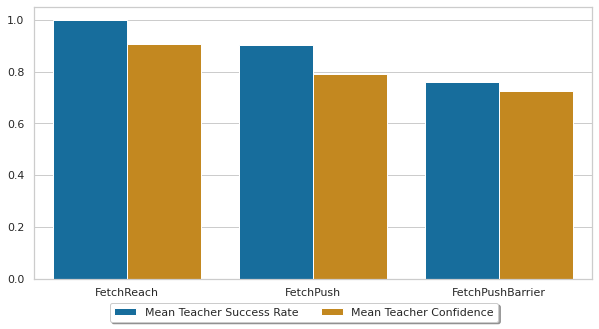
\includegraphics[width=\textwidth]{images/results/ensemble_combined_bar.png}
    \caption[Comparison of the mean success rate and confidence of the teachers.]{Comparison of the mean success rate and confidence of the teachers. For each environment, all three agents that form the ensemble teacher where evaluated on 1000 episodes, to calculate the mean success rate. To calculate the mean confidence, first the best agent of each ensemble, with regards to the success rate, was selected. This agent was evaluated again on 1000 episodes. The environment was initialized with the same seed. For each action, the confidence was calculated using all three agents. The mean of the confidence of all actions is shown here.}
    \label{fig:results:barrier-drq-ensemble-bar}
\end{figure}